\documentclass[a4paper]{article}

\usepackage{graphicx}

\begin{document}

\title{Improving image classification with CNNs by exploiting selectivity in search and training data}

\author{Muhammad Iqbal Tawakal}

\maketitle

\begin{abstract}
This is abstract. To be written later.
\end{abstract}

\section{Introduction}
Since the inception of computer and artificial intelligence field, the problem of obtaining understanding from visual perception has been viewed as a seemingly simple step to solve a more difficult obstacle such as higher-level reasoning and planning. However, this problem surprisingly turns out to be much harder than it is originally anticipated. Forty years later, it still eludes scientist and becomes one of the most highly active field of research.

One class of problem in the computer vision is image classification. That is, given an image or a set of images, determined whether a certain class object present in the image or not. This is usually tackled by using a set of binary classifiers, each trained to classify a single object with specified set of features. Many studies have proposed different ways to extract the most discriminating feature. Some most notably successful features are SIFT \cite{lowe2004sift}, HOG \cite{dalal2005hog}, and LBP \cite{ahonen2006lbp}. However, it still falls short to encode the rich variation of objects in image and progress has been stagnated in the last few years.

A breakthrough comes with, now seminal, paper by Krizhevsky et al \cite{krizhevsky2012} which shows that an algorithm that has been proposed in the early 90s, Convolutional Neural Network (CNN), have staggering performance and beat the last state-of-the-art method with large margin. This is made possible by the combination of the availability of large number of training data (1.2 million training images from ImageNet dataset \cite{deng2009imagenet}) and processing prowess of Graphical Processing Unit (GPU) which can speed up the computation up to 20 times faster. Since then, progress have been made steadily every year, either by using a bigger, larger network or using even more training data.

Event further, we can treat the CNN that has been trained with big dataset with large number of training images as black box feature extractor. Feed an image into the network (after pre-processing step) and it will output features with significantly lower dimension and better separability. It has been showed that these features excel in many vision tasks, ranging from image classification, object detection, and image retrieval \cite{alicvpr2014} even on par with state-of-the-art method with highly engineered features using only simple linear classifier.

This independent course project extends the previous works, specifically on image classification problem. The CNN features is not extracted from the whole image, instead it comes from part of the image. These patches are produced from region proposal algorithm which search for possible object location in the image. These features are then trained with simple linear classifier. In our case, SVM with linear kernel is used. The performance will be assessed using PASCAL VOC 2007 dataset.

The organization for the rest of this report is as follows. The method used will be explained in section \ref{sec:method}. The experiment setup, result and its analysis will be covered in section \ref{sec:experiment}. Finally, section \ref{seg:conclusion} will provide the conclusion and direction for future work.

\section{Method}
\label{sec:method}

\subsection{Convolutional Neural Network}
Convolutional Neural Network (CNN) is one variant of the popular multi-layered neural network. This algorithm first proposed by Yann LeCun for handwritten document classification \cite{lecun}. Two different paradigms than the standard MLP is first, sparse connectivity and shared weights. This ultimately is just a convolution operation of the image with a certain kernel.

\begin{figure}[h]
\centering
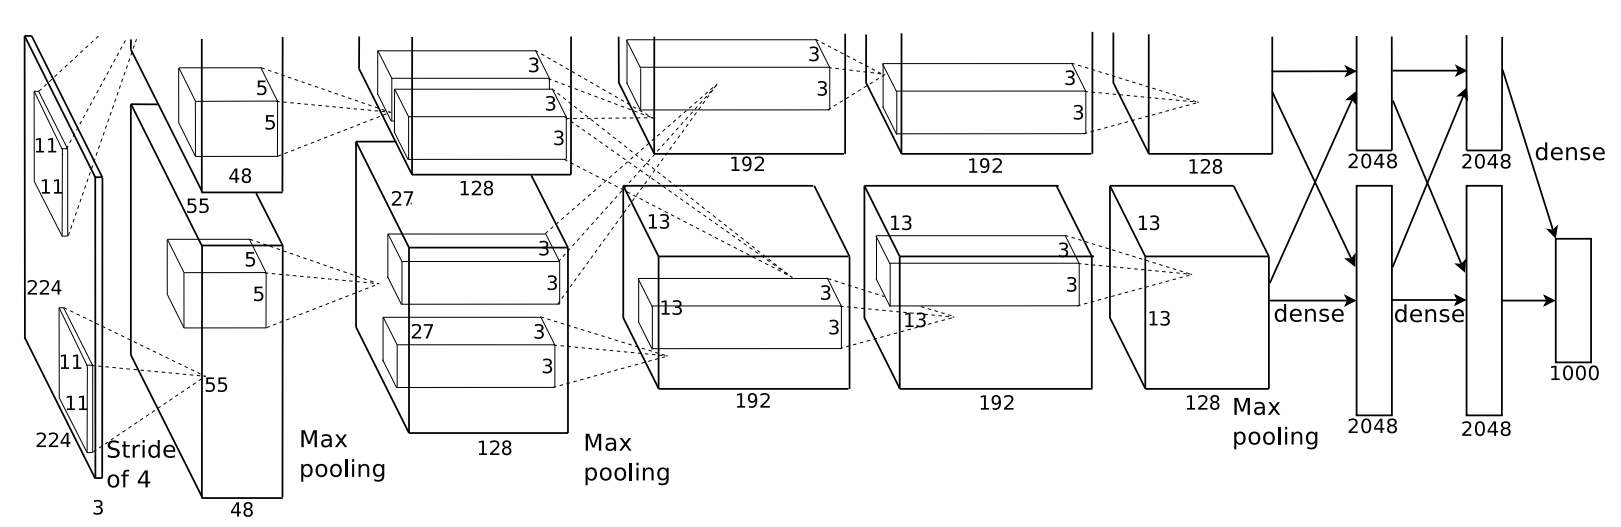
\includegraphics[scale=0.3]{img/alexnet.png}
\caption{AlexNet architecture}
\end{figure}

The architecture, dubbed as AlexNet, and defeat the previous state-of-the-art method by large margin. dropout to reduce overfitting.
This architecture composed of 5 convolutional layer, each followed by a max-pool then a rectified linear unit as its activation function. Equation 1 shows the definition of this function.

\begin{equation}
f(x) = max(0, x)
\end{equation}

For the purpose of this experiment, an implementation called Caffe is used to implements this architecture \cite{jia2013}.

\subsection{Selective Search}
Selective search is a region proposal region proposed by \cite{uva}. The 
Selective search region proposal algorithm works by combining the result of its base segmentation algorithm using different (after some duplicates have been removed) parameter such as, size and color space. It used Felzenszwalb graph segmentation algorithm as its base, before hierarchical grouping procedure is applied. The grouping criterion is based on size, texture, and similarity.

[Insert Image Here]

Another paper which also uses the same algorithm as its base for object detection have discussion of alternative strategy.

\subsubsection{Hard negative mining}

\section{Experiment}
\label{sec:experiment}

\subsection{Dataset}
The dataset used is PASCAL Visual Object Classification (VOC) 2007. This dataset consists of. There are 3 training, validation, and testing dataset.

\subsection{Choosing positive samples for training}
For testing we simply use all regions.
If this value more than a specified threshold, we consider it to be positive samples. Negative samples are 

\subsection{Hard negative mining}
Due to the limitation of memory and computation power, the number of training data must be limited. Hence, hard negative mining strategy is employed. This is also motivated by the facts that the number of positive samples is significantly lower than negative samples.

\subsection{Result}
There are several experiments conducted to test the hypothesis. First, a baseline experiment to reproduce the paper result is conducted. This experiment is conducted by 
The result can be seen on Table \ref{tab:ap}

[Insert Table Here]

\section{Conclusion}
\label{seg:conclusion}

\bibliographystyle{plain}
\bibliography{finalreport}

\end{document}
